\documentclass[12pt, titlepage]{article}

\usepackage{amsmath, mathtools}

\usepackage[round]{natbib}
\usepackage{amsfonts}
\usepackage{amssymb}
\usepackage{graphicx}
\usepackage{colortbl}
\usepackage{xr}
\usepackage{hyperref}
\usepackage{longtable}
\usepackage{xfrac}
\usepackage{tabularx}
\usepackage{float}
\usepackage{siunitx}
\usepackage{booktabs}
\usepackage{multirow}
\usepackage[section]{placeins}
\usepackage{caption}
\usepackage{fullpage}

\hypersetup{
bookmarks=true,     % show bookmarks bar?
colorlinks=true,       % false: boxed links; true: colored links
linkcolor=red,          % color of internal links (change box color with linkbordercolor)
citecolor=blue,      % color of links to bibliography
filecolor=magenta,  % color of file links
urlcolor=cyan          % color of external links
}

\usepackage{array}

\externaldocument{../../SRS/SRS}

\newcounter{mnum}
\newcommand{\mthemnum}{M\themnum}
\newcommand{\mref}[1]{M\ref{#1}}

%% Comments

\usepackage{color}

\newif\ifcomments\commentstrue %displays comments
%\newif\ifcomments\commentsfalse %so that comments do not display

\ifcomments
\newcommand{\authornote}[3]{\textcolor{#1}{[#3 ---#2]}}
\newcommand{\todo}[1]{\textcolor{red}{[TODO: #1]}}
\else
\newcommand{\authornote}[3]{}
\newcommand{\todo}[1]{}
\fi

\newcommand{\wss}[1]{\authornote{blue}{SS}{#1}} 
\newcommand{\plt}[1]{\authornote{magenta}{TPLT}{#1}} %For explanation of the template
\newcommand{\an}[1]{\authornote{cyan}{Author}{#1}}

%% Common Parts

\newcommand{\progname}{ProgName} % PUT YOUR PROGRAM NAME HERE
\newcommand{\authname}{Team \#, Team Name
\\ Student 1 name
\\ Student 2 name
\\ Student 3 name
\\ Student 4 name} % AUTHOR NAMES                  

\usepackage{hyperref}
    \hypersetup{colorlinks=true, linkcolor=blue, citecolor=blue, filecolor=blue,
                urlcolor=blue, unicode=false}
    \urlstyle{same}
                                


\begin{document}

\title{Module Interface Specification for Hairesthetics}

\author{Team 18 \\ Charlotte Cheng
        \\ Marlon Liu
        \\ Senni Tan
        \\ Qiushi Xu
        \\ Hongwei Niu
        \\ Bill Song
}

\date{\today}

\maketitle

\pagenumbering{roman}

\section{Revision History}

\begin{tabularx}{\textwidth}{p{3cm}p{2cm}X}
\toprule {\bf Date} & {\bf Version} & {\bf Notes}\\
\midrule
Jan 17 & 0 & Rev0 MIS\\
\bottomrule
\end{tabularx}

~\newpage

\section{Symbols, Abbreviations and Acronyms}
\begin{tabular}{l l} 
  \toprule		
  \textbf{symbol} & \textbf{description}\\
  \midrule 
  ML & Machine Learning \\
  UI & User Interface\\
  AI & Artificial Intelligence \\
  AR & Augumented Reality \\
  App & Application \\
  API & Application programming interface\\
  REST & Representational state transfer\\
  RGB & Red, Green, Blue \\
  macOS & Operating system developed by Apple Inc \\
  MG & Module Guide \\
  MIS & Module Interface Specification \\
  \bottomrule
\end{tabular}\\
\newline
See SRS Documentation at \href{https://github.com/marlon4dashen/Hairesthetics/blob/main/docs/SRS/SRS.pdf}{/docs/SRS/SRS.pdf}

\newpage

\tableofcontents
\listoftables
\listoffigures

\newpage

\pagenumbering{arabic}

\section{Introduction}

The following document details the Module Interface Specifications for the Hairesthetics application. Hairesthetics is an application that simulates 3D hairstyles.

Complementary documents include the System Requirement Specifications
and Module Guide.  The full documentation and implementation can be
found at \url{https://github.com/marlon4dashen/Hairesthetics}. 

\section{Notation}

The structure of the MIS for modules comes from HoffmanAndStrooper1995,
with the addition that template modules have been adapted from
GhezziEtAl2003. The mathematical notation comes from Chapter 3 of
HoffmanAndStrooper1995. For instance, the symbol:= is used for a
multiple assignment statement and conditional rules follow the form $(c_1
\Rightarrow r_1 | c_2 \Rightarrow r_2 | ... | c_n \Rightarrow r_n )$.

The following table summarizes the primitive data types used by the modules. 

\begin{center}
\renewcommand{\arraystretch}{1.2}
\noindent 
\begin{tabular}{l l p{7.5cm}} 
\toprule 
\textbf{Data Type} & \textbf{Notation} & \textbf{Description}\\ 
\midrule
character & char & a single symbol or digit\\
integer & $\mathbb{Z}$ & a number without a fractional component in (-$\infty$, $\infty$) \\
natural number & $\mathbb{N}$ & a number without a fractional component in [1, $\infty$) \\
real & $\mathbb{R}$ & any number in (-$\infty$, $\infty$)\\
\bottomrule
\end{tabular} 
\end{center}

\noindent
The specification of our modules uses some derived data types: sequences, strings, and tuples. Sequences are lists filled with elements of the same data type. Strings are sequences of characters. Tuples contain a list of values, potentially of different types. In addition, our modules use functions, which are defined by the data types of their inputs and outputs. Local functions are described by giving their type signature followed by their specification.

\section{Module Decomposition}

This section provides an overview of the module design. Modules are summarized
in a hierarchy decomposed by secrets in Table \ref{TblMH}. The modules listed
below, which are leaves in the hierarchy tree, are the modules that will
actually be implemented.

\begin{description}
\item [\refstepcounter{mnum} \mthemnum \label{mHH}:] Controller Module
\item [\refstepcounter{mnum} \mthemnum \label{mHH}:] Facial Recognition Module
\item [\refstepcounter{mnum} \mthemnum \label{mHH}:] Hair Color Module
\item [\refstepcounter{mnum} \mthemnum \label{mHH}:] Hair Style Module
\item [\refstepcounter{mnum} \mthemnum \label{mHH}:] Salon Recommendation Module
\item [\refstepcounter{mnum} \mthemnum \label{mHH}:] ML Model Module
\item [\refstepcounter{mnum} \mthemnum \label{mHH}:] Utility Module
\item [\refstepcounter{mnum} \mthemnum \label{mHH}:] Hair Color View Module
\item [\refstepcounter{mnum} \mthemnum \label{mHH}:] Hair Style View Module
\item [\refstepcounter{mnum} \mthemnum \label{mHH}:] Salon Recommendation Interface Module
\item [\refstepcounter{mnum} \mthemnum \label{mHH}:] Home View Module
\item [\refstepcounter{mnum} \mthemnum \label{mHH}:] Camera Module
\item [\refstepcounter{mnum} \mthemnum \label{mHH}:] Error View Module
\end{description}

\begin{table}[H]
\centering
\begin{tabular}{p{0.3\textwidth} p{0.6\textwidth}}
\toprule
\textbf{Level 1} & \textbf{Level 2}\\
\midrule

{Hardware-Hiding Module} & M13 \\
\midrule

\multirow{7}{0.3\textwidth}{Behaviour-Hiding Module}
& M1\\
& M2\\
& M3\\
& M4\\
& M5\\
& M8\\
& M9\\
& M10\\
& M11\\
& M13\\
\midrule

\multirow{2}{0.3\textwidth}{Software Decision Module} & M6 \\  & M7\\
\bottomrule

\end{tabular}
\caption{Module Hierarchy}
\label{TblMH}
\end{table}

\subsection{UML Diagram}
\begin{center}
\begin{figure}[]
% \graphicspath{ {component_diagram.jpg} }
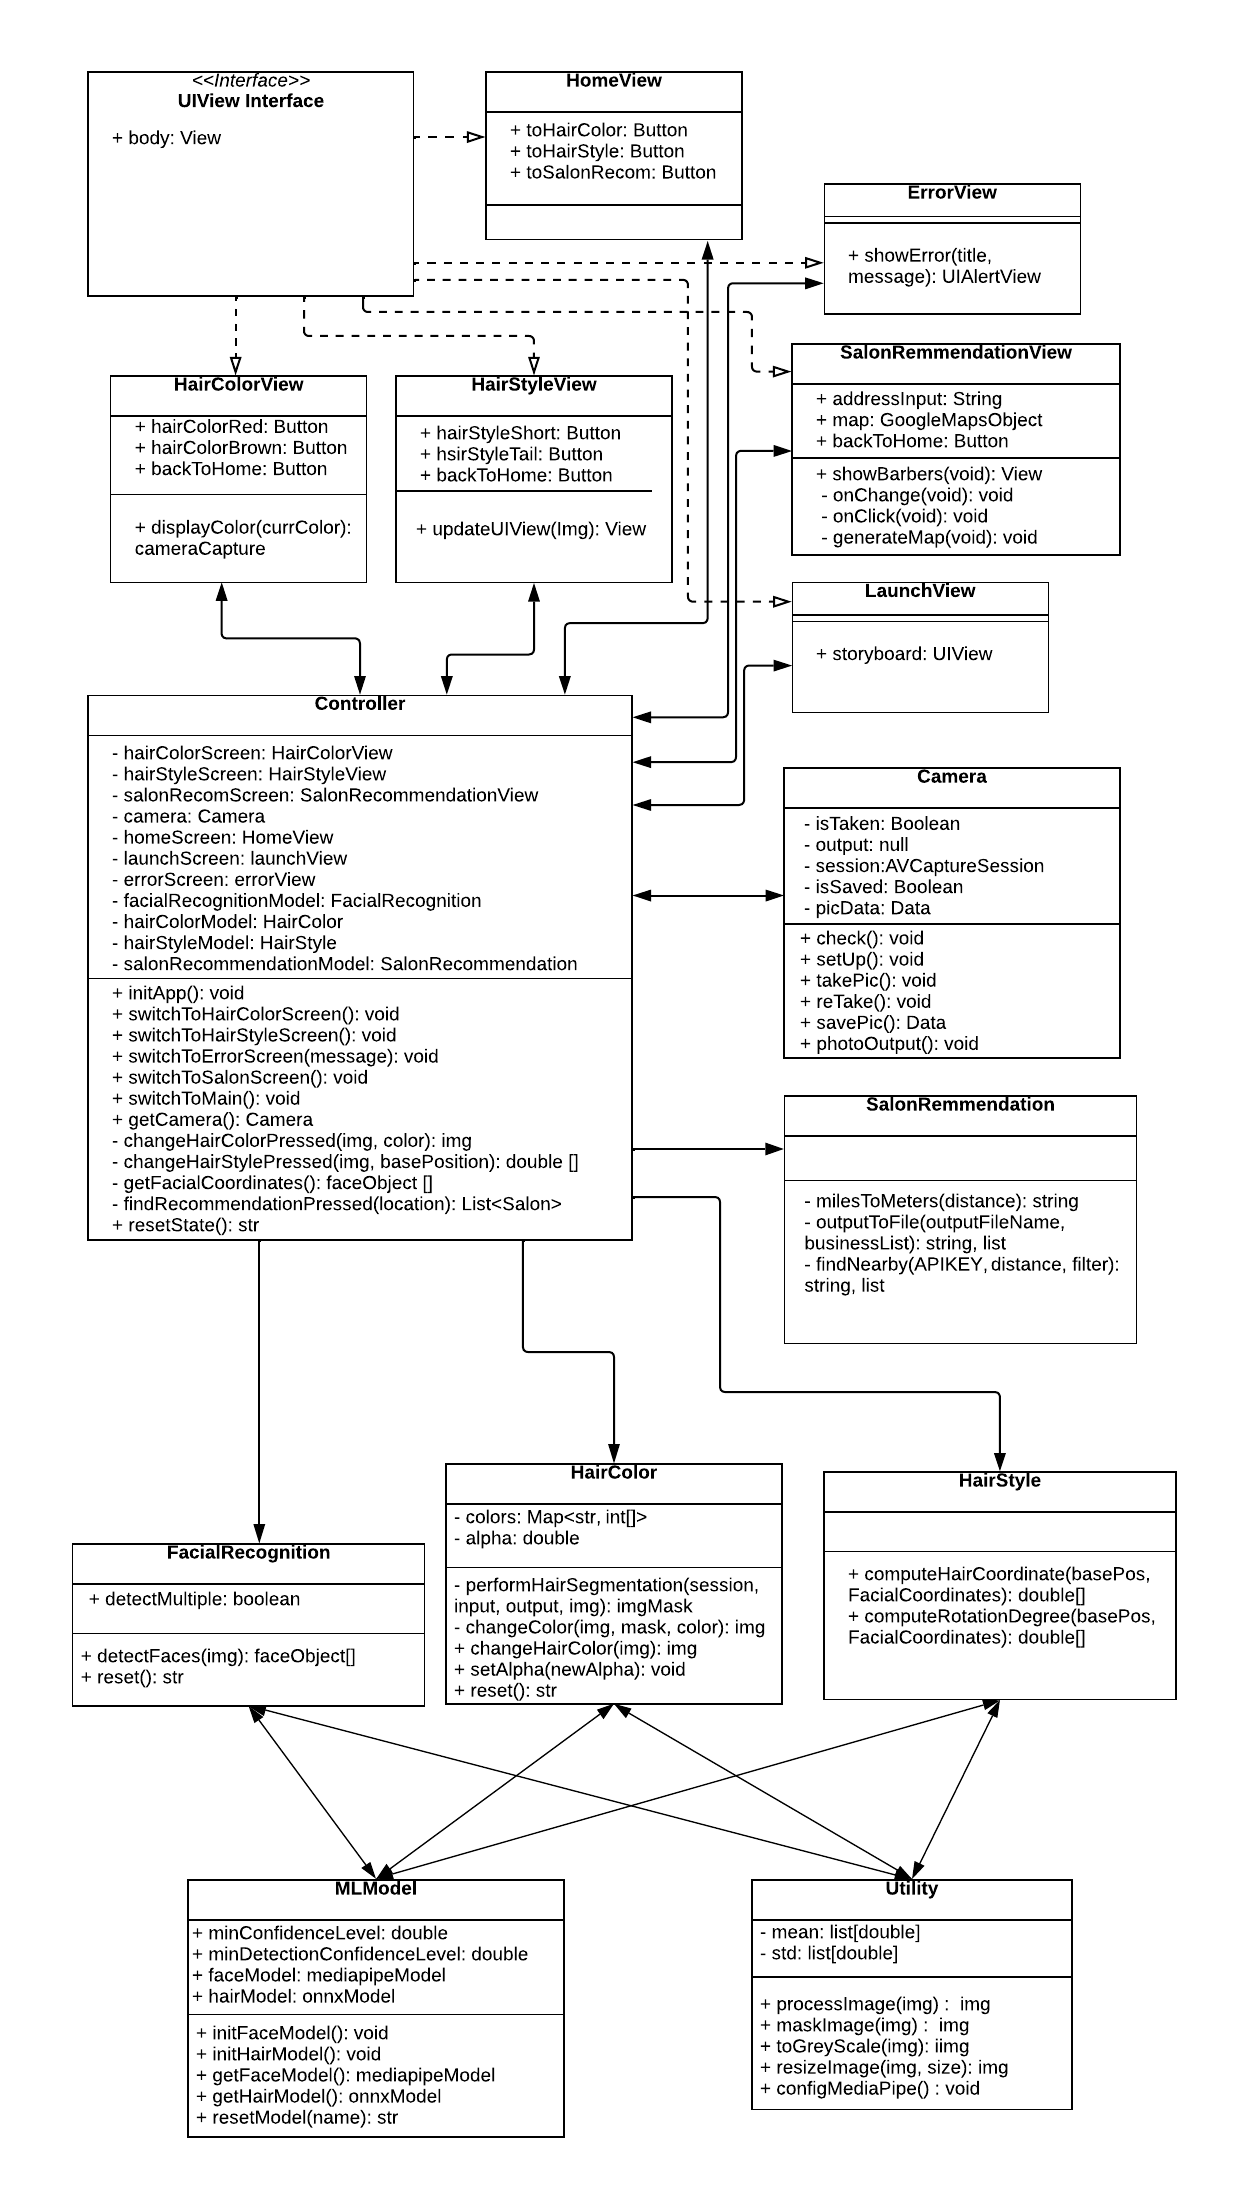
\includegraphics[width=0.8\textwidth, scale=0.8, keepaspectratio]{Design/SoftArchitecture/UML.png}
\caption{UML Diagram}
\label{FigUH} 
\end{figure}
\end{center}

~\newpage

\section{MIS of Controller Module}

\subsection{Module}
M1 - Controller \\
Abstract Data Type Module

\subsection{Uses}
FacialRecognition (M2) \\
HairColor (M3) \\
HairStyle (M4) \\
SalonRecommendation (M5) \\
HairColorView (M8) \\
HairStyleView (M9) \\
SalonRecommendationView (M10) \\
HomeView (M11) \\
ErrorView (M13) \\
Camera (M12) \\

\subsection{Syntax}

\subsubsection{Exported Constants}

\subsubsection{Exported Access Programs}

\begin{center}
\begin{tabular}{p{5cm} p{3cm} p{3cm} p{2cm}}
\hline
\textbf{Name} & \textbf{In} & \textbf{Out} & \textbf{Exceptions} \\
\hline
initApp & - & - & - \\
switchToHairColorScreen & - & - & - \\
switchToHairStyleScreen & - & - & - \\
switchToErrorScreen & string & - & - \\
switchToSalonScreen & - & - & - \\
switchToMain & - & - & - \\
getCamera & - & Camera & - \\
resetState & & & \\
\hline
\end{tabular}
\end{center}

\subsection{Semantics}

\subsubsection{State Variables}
hairColorScreen := HairColorView \\
hairStyleScreen := HairStyleView \\
salonRecomScreen := SalonRecommendationView \\
camera := Camera \\
homeScreen := HomeView \\
launchScreen := launchView \\
errorScreen := errorView \\
facialRecognitionModel := FacialRecognition \\
hairColorModel := HairColor \\
hairStyleModel := HairStyle \\
salonRecommendationModel := SalonRecommendation \\
currentView := homeScreen

\subsubsection{Environment Variables}

\subsubsection{Assumptions}

\subsubsection{Access Routine Semantics}

\noindent initApp():
\begin{itemize}
\item transition: \\
switchScreen(launchScreen) \\
currentView.display()
\item output: 
\item exception:
\end{itemize}

\noindent switchToHairColorScreen():
\begin{itemize}
\item transition: switchScreen(hairColorScreen) 
\item output:
\item exception:
\end{itemize}

\noindent switchToHairStyleScreen():
\begin{itemize}
\item transition: switchScreen(hairStyleScreen) 
\item output:
\item exception:
\end{itemize}

\noindent switchToErrorScreen(message):
\begin{itemize}
\item transition: switchScreen(errorScreen) 
\item output:
\item exception: 
\end{itemize}

\noindent switchToSalonScreen():
\begin{itemize}
\item transition: switchScreen(salonScreen) 
\item output:
\item exception:
\end{itemize}

\noindent switchToMain():
\begin{itemize}
\item transition: switchScreen(homeScreen) 
\item output:
\item exception: 
\end{itemize}

\noindent getCamera():
\begin{itemize}
\item transition:
\item output: camera
\item exception:
\end{itemize}

\noindent resetState():
\begin{itemize}
\item transition: currentView.clear()
\item output: 
\item exception: 
\end{itemize}

\subsubsection{Local Functions}

\noindent getFacialCoordinates(img):
\begin{itemize}
\item input: \\
img - inputImage 
\item transition:
\item output: \\
faces := facialRecognitionModel.detectFaces(img) \\
return faces - faceObject[]
\item exception:
\end{itemize}

\noindent changeHairColorPressed(img, color):
\begin{itemize}
\item input: \\
img - inputImage \\
color - rgb values
\item transition:
\item output: \\
outImg := hairColorModel.changeHairColor(img, color) \\
return outImg - image with chose hair color
\item exception:
\end{itemize}

\noindent changeHairStylePressed(img, basePosition):
\begin{itemize}
\item input: \\
img - inputImage \\
basedPosition - camera base position
\item transition:
\item output: \\
coordinates := getFacialCoordinates(img) \\
rotationDegrees := hairStyleModel.computeRotationDegree(coordinates) \\
return rotationDegrees - double[]
\item exception:
\end{itemize}

\noindent switchScreen(view):
\begin{itemize}
currentView.reset() \\
view.display() \\
currentView := view \\
\end{itemize}

\noindent binding():
\begin{itemize}
HairColorView.backToHomeButton.event.pressed(switchScreen(homeScreen)) \\
HairStyleView.backToHomeButton.event.pressed(switchScreen(homeScreen)) \\
SalonRecommendationView.backToHomeButton.event.pressed(switchScreen(homeScreen)) \\
ErrorView.backToHomeButton.event.pressed(switchScreen(homeScreen)) \\
HairColorView.selectedColor.event.pressed(changeHairColorPressed(img, color)) \\
HairStyleView.previousHairStyle.event.pressed(changeHairStylePressed(img, basePosition)) \\
HairStyleView.nextHairStyle.event.pressed(changeHairStylePressed(img, basePosition)) \\
\end{itemize}

\newpage
\section{MIS of Facial Recognition Module}
\subsection{Module}
M2 - FacialRecognition\\
Abstract Object Module

\subsection{Uses}
MLModel (M6) \\
Utility (M7)

\subsection{Syntax}

\subsubsection{Exported Constants}
\subsubsection{Exported Access Programs}

\begin{center}
\begin{tabular}{p{4cm} p{3cm} p{4cm} p{4cm}}
\hline
\textbf{Name} & \textbf{In} & \textbf{Out} & \textbf{Exceptions} \\
\hline
detectFaces & image & list of face objects & InterruptException \\
detectMultipleFaces & boolean &  &  \\
reset & & string & \\
\hline
\end{tabular}
\end{center}

\subsection{Semantics}

\subsubsection{State Variables}
detectMultiple := true

\subsubsection{Environment Variables}

\subsubsection{Assumptions}

\subsubsection{Access Routine Semantics}
\noindent detectFaces(img):
\begin{itemize}
\item transition:
\item output: \\
processedImage = Utility.toGreyScale(img) \\
if detectMultiple == true $=>$ MLModel.getFaceModel().process(processedImage)\\
if detectMultiple == false $=>$ MLModel.getFaceModel().process(processedImage, max\_faces=1) \\
return results - a list of face objects detected in the input image
\begin{center}
\begin{figure}[H]
% \graphicspath{ {component_diagram.jpg} }
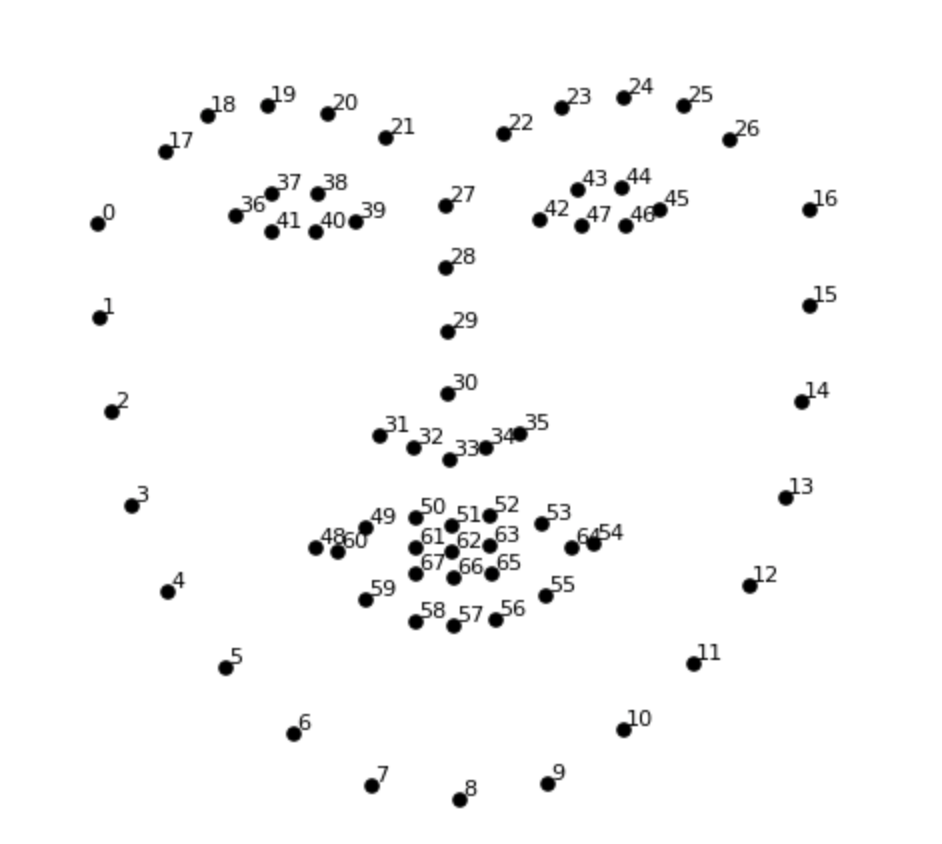
\includegraphics[scale=0.5]{Design/SoftDetailedDes/face_mesh.png}
\caption{Face Landmarks within a face object}
\label{Fig_UseHierarchy} 
\end{figure}
\end{center}
\item exception: InterruptException := action terminated by the user
\end{itemize}

\noindent detectMultipleFaces(status):
\begin{itemize}
\item transition: detectMultiple := status
\item output: 
\item exception: 
\end{itemize}

\noindent reset():
\begin{itemize}
\item transition: 
\item output: message $=>$ MLModel.reset(hair)
\item exception: 
\end{itemize}

\subsubsection{Local Functions}
None

\newpage
\section{MIS of Hair Color Module}
\subsection{Module}
M3 - HairColor Module\\
Abstract Object Module

\subsection{Uses}
MLModel (M6) \\
Utility (M7)

\subsection{Syntax}

\subsubsection{Exported Constants}
\subsubsection{Exported Access Programs}

\begin{center}
\begin{tabular}{p{4cm} p{3cm} p{4cm} p{4cm}}
\hline
\textbf{Name} & \textbf{In} & \textbf{Out} & \textbf{Exceptions} \\
\hline
% performHairSegmentation & onnx\_session, list[int], list[int], image & image & InterruptException \\
% changeColor & image, image, string & image &  KeyErrorException\\
changeHairColor & image, string & image & KeyErrorException \\
setAlpha & double & & \\
reset & & string & \\
\hline
\end{tabular}
\end{center}

\subsection{Semantics}

\subsubsection{State Variables}
colors - Map$<$str, int[]$>$ - a mapping between the name of color and their rgb values \\
alpha - double - represents the ratio between the original image and the masked image

\subsubsection{Environment Variables}

\subsubsection{Assumptions}

\subsubsection{Access Routine Semantics}

\noindent changeHairColor(image, color):
\begin{itemize}
\item input: \\ image - the copy of an original image \\ color - the chosen hair color
\item transition: N/A
\item output:\\
hairModelSession = utility.getHairModel() \\
mask = performHairSegmentation(hairModelSession, hairModelSession.inputName, hairModelSession.output image) - the image where the hair detected by the model is masked. \\
outputImg = changeColor(image, mask, color) \\
return outputImg - an image where the hair color of each person is changed to the specified color
\item exception: InterruptException - the prediction and masking process is interrupted by the user
\end{itemize}

\noindent setAlpha(newAlpha):
\begin{itemize}
\item input: newAlpha - double - input alpha value for update
\item transition: alpha := newAlpha - update the alpha value
\item output: N/A
\item exception: N/A
\end{itemize}

\noindent reset():
\begin{itemize}
\item transition:
\item output: message $=>$ MLModel.reset(hair)
\item exception: 
\end{itemize}

\subsubsection{Local Functions}

\noindent performHairSegmentation(session, input, output, image):
\begin{itemize}
\item input: session  - the onnx inference session that contains the input model\\
input - list of integer - the input shape of the image\\
output - list of integer - the expected output shape\\
image - the copy of an original image
\item transition: N/A
\item output: mask - hair mask.
\begin{center}
\begin{figure}[H]
% \graphicspath{ {component_diagram.jpg} }

\includegraphics[width=0.5\textwidth]{Design/SoftDetailedDes/hair_mask.png}
\caption{Hair Mask after running the pre-trained hair segmentation model}
\label{Fig_UseHierarchy} 
\end{figure}
\end{center}
\item exception: KeyErrorException - the specified color is not in the color map
\end{itemize}

 \noindent changeColor(img, mask, color):
\begin{itemize}
\item input: img - the original image, mask - the masked image generated from hair segmentation, color - color's name as a string
\item transition: N/A
\item output: an image where the original image is mixed with the masked image.
\item exception: KeyErrorException - the specified color is not in the color map
\end{itemize}

\newpage
\section{MIS of Hair Style Module}
\subsection{Module}
M9 - FacialRecognition\\
Abstract Object Module

\subsection{Uses}
MLModel (M6) \\
Utility (M7)

\subsection{Syntax}

\subsubsection{Exported Constants}
\subsubsection{Exported Access Programs}

\begin{center}
\begin{tabular}{p{4cm} p{3cm} p{4cm} p{4cm}}
\hline
\textbf{Name} & \textbf{In} & \textbf{Out} & \textbf{Exceptions} \\
\hline
computeHairCoordinate & list[double], list[double] & list[double] &  \\
computeRotationDegree & list[double], list[double] & list[double] &  \\
\hline
\end{tabular}
\end{center}

\subsection{Semantics}

\subsubsection{State Variables}

\subsubsection{Environment Variables}

\subsubsection{Assumptions}

\subsubsection{Access Routine Semantics}
\noindent computeHairCoordinate(basePosition, facialCoordinates):
\begin{itemize}
\item input: basePosition - the basePosition of the camera setting in a tuple \\
facialCoordinates - a list of coordinates of the facial features
\item transition: N/A
\item output: output the desired position to place the hairstyle centered at a coordinate, computed based on the base position and facial coordinates.
\item exception: InterruptException := action terminated by the user
\end{itemize}

\noindent computeRotationDegree(basePosition, facialCoordinates):
\begin{itemize}
\item input: basePosition - the basePosition of the camera setting in a tuple \\
facialCoordinates - a list of coordinates of the facial features
\item transition: N/A
\item output: output the desired rotation of the hairstyle when being placed on the user's face, computed based on the base position and facial coordinates.
\end{itemize}

\subsubsection{Local Functions}
 
\newpage
\section{MIS of Salon Recommendation Module} \label{Module} 

\subsection{Module}
M5: Salon Recommendation Module \\
Abstract Object Module


\subsection{Uses}


\subsection{Syntax}

\subsubsection{Exported Constants}

\subsubsection{Exported Access Programs}

\begin{center}
\begin{tabular}{p{4cm} p{3cm} p{4cm} p{4cm}}
\hline
\textbf{Name} & \textbf{In} & \textbf{Out} & \textbf{Exceptions} \\
\hline
milesToMeter  & int &  int  & - \\
outputToFile & string, list & file & - \\
findNearby & string, list & string, list & IndexOutOfRange \\
\hline
\end{tabular}
\end{center}

\subsection{Semantics}

\subsubsection{State Variables}

\subsubsection{Environment Variables}

\subsubsection{Assumptions}

\subsubsection{Access Routine Semantics}

\noindent milesToMeter(distance):
\begin{itemize}
\item input: The input to the function would be the distance between the two points in miles.
\item transition:  
\item output: output the distance between two locations from miles to meters. used to give the user more precise measurements, or to conform to international standards. 
\item exception: InvalidValueException - The value is negative or irational numbers 
\end{itemize}

\noindent outputToFile(outputFileName, businessList):
\begin{itemize}
\item input: The input to the function would be the self defined output filename and the generated list after sorting the salon choices.
\item transition:  
\item output: output the file that stores the customized hair salon information after sorting. 
\end{itemize}

\noindent findNearby(APIKEY, distance, filter):
\begin{itemize}
\item input: The input to the function would be the google API KEY, the distance user want to search for, and the filter information used to filter hair salons.
\item transition:  
\item output: output the sorted business list
\item exception: IndexOutOfRange: the value of distance is invalid
\end{itemize}
\subsubsection{Local Functions}

\newpage
\section{MIS of ML Model Module}
\subsection{Module}
M6 - MLModel\\
Abstract Object Module

\subsection{Uses}
Mediapipe (External Module) \\
Onnx (External Module) \\

\subsection{Syntax}

\subsubsection{Exported Constants}

\subsubsection{Exported Access Programs}

\begin{center}
\begin{tabular}{p{4cm} p{3cm} p{4cm} p{4cm}}
\hline
\textbf{Name} & \textbf{In} & \textbf{Out} & \textbf{Exceptions} \\
\hline
initFaceModel & &  & InterruptException \\
initHairModel & &  &  \\
getFaceModel & & mediapipeModel & \\
getHairModel & & onnxModel & \\
resetModel & string & string & \\
\hline
\end{tabular}
\end{center}

\subsection{Semantics}

\subsubsection{State Variables}
minConfidenceLevel := 0.5 \\
minDetectionConfidence := 0.5 \\
modelFilePath := filePath (path to the pre-trained model) \\
faceModel := null \\
hairModel := null


\subsubsection{Environment Variables}

\subsubsection{Assumptions}

\subsubsection{Access Routine Semantics}
\noindent initFaceModel():
\begin{itemize}
\item transition: faceModel := mediapipe.FaceMesh(minConfidenceLevel, minDetectionConfidence)
\item output: 
\item exception:
\end{itemize}

\noindent initHairModel():
\begin{itemize}
\item transition: 
hairModel := onnxruntime.InferenceSession(modelFilePath) \\
\item output: 
\item exception: 
\end{itemize}

\noindent getFaceModel():
\begin{itemize}
\item transition:
\item output: faceModel
\item exception:
\end{itemize}

\noindent getHairModel():
\begin{itemize}
\item transition:
\item output: hairModel
\item exception: 
\end{itemize}

\noindent resetModel(name):
\begin{itemize}
\item transition: \\
if name == "face" then initFaceModel() \\
else if name == "hair", then initHairModel()
\item output: 
\item exception: 
\end{itemize}

\subsubsection{Local Functions}

\newpage
\section{MIS of Utility Module}
\subsection{Module}
M7 - Utility Module\\
Library

\subsection{Uses}
OpenCV (External Module)
Numpy (External Module)

\subsection{Syntax}

\subsubsection{Exported Constants}
\subsubsection{Exported Access Programs}

\begin{center}
\begin{tabular}{p{4cm} p{3cm} p{4cm} p{4cm}}
\hline
\textbf{Name} & \textbf{In} & \textbf{Out} & \textbf{Exceptions} \\
\hline
processImage & image, list[int] & tensor & illegalArgumentException \\
maskImage & image, image & image  & illegalArgumentException \\
toGreyScale & image & image & \\
resizeImage & image, list[int] & image & illegalArgumentException \\
\hline
\end{tabular}
\end{center}

\subsection{Semantics}

\subsubsection{State Variables}
mean - list[double] - the mean values of trained images, used to normalize the images \\
std - list[double] - the standard deviation values of trained images, used to normalize the images \\

\subsubsection{Environment Variables}

\subsubsection{Assumptions}

\subsubsection{Access Routine Semantics}
\noindent processImage(image, input\_size):
\begin{itemize}
\item input: image - the original input image in the form of 3-dimensional array, input\_size - a tuple represents the input size the ML model requires
\item transition: N/A
\item output: \\
OpenCV.convertColor(image, BGR2RGB) - convert the image to RGB format \\ resizeImage(image, input\_size) - convert image to input size \\
image = (image / 255 - mean) / std - normalize the image \\
Numpy.expandDimension(image, axis=0) - expand one dimension to a tensor \\
output a image tensor ready for process with the model
\item exception: illegalArgumentException - illegal input size for resizing
\end{itemize}

\noindent maskImage(original\_img, mask):
\begin{itemize}
\item input: original\_img - the original image in the form of 3-dimensional array, mask - the masked image in the form of 3-dimensional array with same dimension as original
\item transition: N/A
\item output: \\
OpenCV.bitwise\_or(original\_img, original\_img, mask) - apply masking to the original image with the given mask. \\
output a masked image.
\item exception: illegalArgumentException - original image has different size from the masked image.
\end{itemize}

\noindent toGreyScale(image):
\begin{itemize}
\item input: image - the input image to be converted to grey scale
\item transition: N/A
\item output: \\
OpenCV.convertColor(image, BGR2GRAY) - convert the input image to an grey scale image \\
output the greyscaled image
\item exception: 
\end{itemize}

\noindent resizeImage(image, shape):
\begin{itemize}
\item input: image - the input image \\
shape - a tuple represents the width / height to be reshaped into.
\item transition: N/A
\item output: \\
Numpy.reshape(image, shape) - reshape the image \\
output an reshaped image 
\item exception: illegalArgumentException - illegal input size for resizing
\end{itemize}

\subsubsection{Local Functions}
None

\newpage
\section{MIS of Hair Color View Module} \label{Module} 
\subsection{Module}
M8 - HairColorView\\
Abstract Object Module

\subsection{Uses}
None

\subsection{Syntax}
\subsubsection{Exported Constants}
None

\subsubsection{Exported Access Programs}
\begin{center}
\begin{tabular}{p{4cm} p{3cm} p{4cm} p{4cm}}
\hline
\textbf{Name} & \textbf{In} & \textbf{Out} & \textbf{Exceptions} \\
\hline
buttonActionRed &  & updateCameraView & - \\
buttonActionBrown &  & updateCameraView & - \\
buttonActionBackToHome &  & backToHomePage & - \\
\hline
\end{tabular}
\end{center}

\subsection{Semantics}

\subsubsection{State Variables}
None

\subsubsection{Environment Variables}
Screen, Camera, Buttons

\subsubsection{Assumptions}
None

\subsubsection{Access Routine Semantics}

\noindent buttonActionRed():
\begin{itemize}
\item transition: None 
\item output: the camera view with user's hair color changed by calling Local function updateHairColor(red).
\item exception: None
\end{itemize}

\noindent buttonActionBrown():
\begin{itemize}
\item transition: None 
\item output: the camera view with user's hair color changed by calling Local function updateHairColor(Brown).
\item exception: None
\end{itemize}

\noindent buttonActionBackToHome():
\begin{itemize}
\item transition: None 
\item output: Go back to home page interface.
\item exception: None
\end{itemize}

\subsubsection{Local Functions}
\noindent updateHairColor(color):
\begin{itemize}
\item transition: None 
\item output: the camera view with user's hair color changed.
\item exception: None
\end{itemize}

\newpage
\section{MIS of Hair Style View Module} \label{Module} 
\subsection{Module}
M9 - HairStyleView\\
Abstract Object Module

\subsection{Uses}
HairStyleModule 

\subsection{Syntax}
\subsubsection{Exported Constants}
None

\subsubsection{Exported Access Programs}
\begin{center}
\begin{tabular}{p{4cm} p{3cm} p{4cm} p{4cm}}
\hline
\textbf{Name} & \textbf{In} & \textbf{Out} & \textbf{Exceptions} \\
\hline
buttonActionShort &  & updateCameraView & - \\
buttonActionTail &  & updateCameraView & - \\
upDateCoordinate &  & updateCoorinates and angle & - \\
buttonActionBackToHome &  & backToHomePage & - \\
\hline
\end{tabular}
\end{center}

\subsection{Semantics}

\subsubsection{State Variables}
Double[][]: coordinates(Represent the coordinates to put the hair model)
Double: A]angle(Represent the angle that the hair model needs to turn)

\subsubsection{Environment Variables}
Screen, Camera, Buttons

\subsubsection{Assumptions}
None

\subsubsection{Access Routine Semantics}

\noindent updateCoordinate():
\begin{itemize}
\item transition: coordinates = HairStyleModule.getCoordinates()  
\item output: None
\item exception: None
\end{itemize}

\noindent updateAngle():
\begin{itemize}
\item transition: coordinates = HairStyleModule.getAngle()  
\item output: None
\item exception: None
\end{itemize}

\noindent buttonActionShort():
\begin{itemize}
\item transition: None 
\item output: the camera view with user's hair style changed by calling Local function upDateHairColor(Short).
\item exception: None
\end{itemize}

\noindent buttonActionTail():
\begin{itemize}
\item transition: None 
\item output: the camera view with user's hair style changed by calling Local function upDateHairColor(Tail).
\item exception: None
\end{itemize}

\noindent buttonActionBackToHome():
\begin{itemize}
\item transition: None 
\item output: Go back to the home page interface.
\item exception: None
\end{itemize}

\subsubsection{Local Functions}
\noindent updateHairStyle(style, coordinates, angle):
\begin{itemize}
\item transition: None 
\item output: the camera view with user's hair style changed.
\item exception: None
\end{itemize}
  
\newpage
\section{MIS of Salon Recommendation View Module} \label{Module}
\subsection{Module}
M10 - SalonRecommendationView
Abstract Object Module

\subsection{Uses}
None

\subsection{Syntax}
\subsubsection{Exported Constants}
None

\subsubsection{Exported Access Programs}
\begin{center}
\begin{tabular}{p{4cm} p{3cm} p{4cm} p{4cm}}
\hline
\textbf{Name} & \textbf{In} & \textbf{Out} & \textbf{Exceptions} \\
\hline
showBarbers & void & View &  \\
\hline
\end{tabular}
\end{center}

\subsection{Semantics}

\subsubsection{State Variables}
addressInput: String \\
map: GoogleMapsObject \\
backToHome: UINavigationButton

\subsubsection{Environment Variables}
Screen 

\subsubsection{Assumptions}
The map object is successfully generated from GoogleMap API before the showBarbers function is called.

\subsubsection{Access Routine Semantics}

\noindent showBarbers():
\begin{itemize}
\item transition: None
\item output: out := View 
\item exception: None
\end{itemize}

\subsubsection{Local Functions}
\noindent onChange(event):
\begin{itemize}
\item transition: addressInput := event.text 
\item output: out := None
\item exception: None
\end{itemize}

\noindent onClick():
\begin{itemize}
\item transition: None 
\item output: out := navigate back to home page
\item exception: None
\end{itemize}

\noindent generateMap():
\begin{itemize}
\item transition: map := new GoogleMapsObject from Google Map API 
\item output: out := None
\item exception: None
\end{itemize}

\section{MIS of Home View Module}
\subsection{Module}
M11 - HomeView Module\\
UIView Module

\subsection{Uses}
Camera (M13) \\
SwiftUI (External Module) \\
RealityKit (External Module) \\
ARKit (External Module) \\

\subsection{Syntax}

\subsubsection{Exported Constants}
\subsubsection{Exported Access Programs}

\subsection{Semantics}

\subsubsection{State Variables}
body - View - View of the home interface, a swift object.
currentMode - String - A string that describes current mode \\
toHairColor - UIButton - Navigate to Haircolor view\\
toHairStyle - UIButton - Navigate to Hairstyle view\\
toSalonRecom - UIButton - Navigate to Salon Recommendation view\\

\subsubsection{Environment Variables}

\subsubsection{Assumptions}

\subsubsection{Access Routine Semantics}

\subsubsection{Local Functions}

\newpage
\section{MIS of Error View Module} \label{Module} 
\subsection{Module}
M12 - ErrorView
Abstract Object Module
\subsection{Uses}
None

\subsection{Syntax}
\subsubsection{Exported Constants}
None

\subsubsection{Exported Access Programs}
\begin{center}
\begin{tabular}{p{4cm} p{3cm} p{4cm} p{4cm}}
\hline
\textbf{Name} & \textbf{In} & \textbf{Out} & \textbf{Exceptions} \\
\hline
showError & String, String & UIAlertView & - \\
\hline
\end{tabular}
\end{center}

\subsection{Semantics}

\subsubsection{State Variables}
None

\subsubsection{Environment Variables}
Screen

\subsubsection{Assumptions}
None

\subsubsection{Access Routine Semantics}

\noindent showError(title, message):
\begin{itemize}
\item transition: None 
\item output: the UIAlertView with the input title and the input message 
\item exception: None
\end{itemize}

\subsubsection{Local Functions}
None

\newpage
\section{MIS of Camera Model Module}
\subsection{Module}
M13 - CameraModel\\
Abstract Object Module

\subsection{Uses}
AVCapture (External Module)\\

\subsection{Syntax}

\subsubsection{Exported Constants}

\subsubsection{Exported Access Programs}

\begin{center}
\begin{tabular}{p{4cm} p{3cm} p{4cm} p{4cm}}
\hline
\textbf{Name} & \textbf{In} & \textbf{Out} & \textbf{Exceptions} \\
\hline
Check & &  & AVCaptureRequestDenial \\
setUp & &  & AVCaptureConfigureError \\
takePic & &  & \\
reTake & &  & \\
savePic &  & Data & UIImageWriteToSavedPhotosAlbumException \\
photoOutput &  &  & \\
\hline
\end{tabular}
\end{center}

\subsection{Semantics}

\subsubsection{State Variables}
AVCapturePhotoCaptureDelegate := \{ \\
isTaken := false \\
output := null \\
session := AVCaptureSession()\\
alert := false\\
isSaved := false\\
picData - Data - stores camera session image data\\
\}\\

\subsubsection{Environment Variables}

\subsubsection{Assumptions}

\subsubsection{Access Routine Semantics}
\noindent Check():
\begin{itemize}
\item transition: AVCaptureDevice.authorizationStatus(for: .video) ? setUp() : AVCaptureDevice.requestAccess(for: .video)
\item output: 
\item exception: AVCaptureRequestDenial
\end{itemize}

\noindent setUp():
\begin{itemize}
\item transition: AVCaptureDevice := AVCaptureDevice.default(.builtInWideAngleCamera, for: .video) 
\item output: 
\item exception: AVCaptureConfigureError
\end{itemize}

\noindent takePic():
\begin{itemize}
\item transition: \\  
isTaken := !self.isTaken\\
output.capturePhoto := (with: AVCapturePhotoSettings(), delegate: self)
\item output: 
\item exception:
\end{itemize}

\noindent reTake():
\begin{itemize}
\item transition: \\  
isTaken := !self.isTaken\\
isSaved := false\\
self.output.capturePhoto := (with: AVCapturePhotoSettings(), delegate: self)
\item output: 
\item exception:
\end{itemize}

\noindent savePic():
\begin{itemize}
\item transition: \\  
isSaved := true\\
\item output: picData
\item exception: UIImageWriteToSavedPhotosAlbumException
\end{itemize}

\noindent photoOutput():
\begin{itemize}
\item transition: \\  
picData := AVCapturePhotoOutput.photo.fileDataRepresentation()
\item output: 
\item exception:
\end{itemize}

\subsubsection{Local Functions}
\bibliographystyle {plainnat}
\bibliography {../../../refs/References}

\newpage

\section{Appendix} \label{Appendix} 

\end{document}